% Created by tikzDevice version 0.12.3.1 on 2021-05-21 22:28:09
% !TEX encoding = UTF-8 Unicode
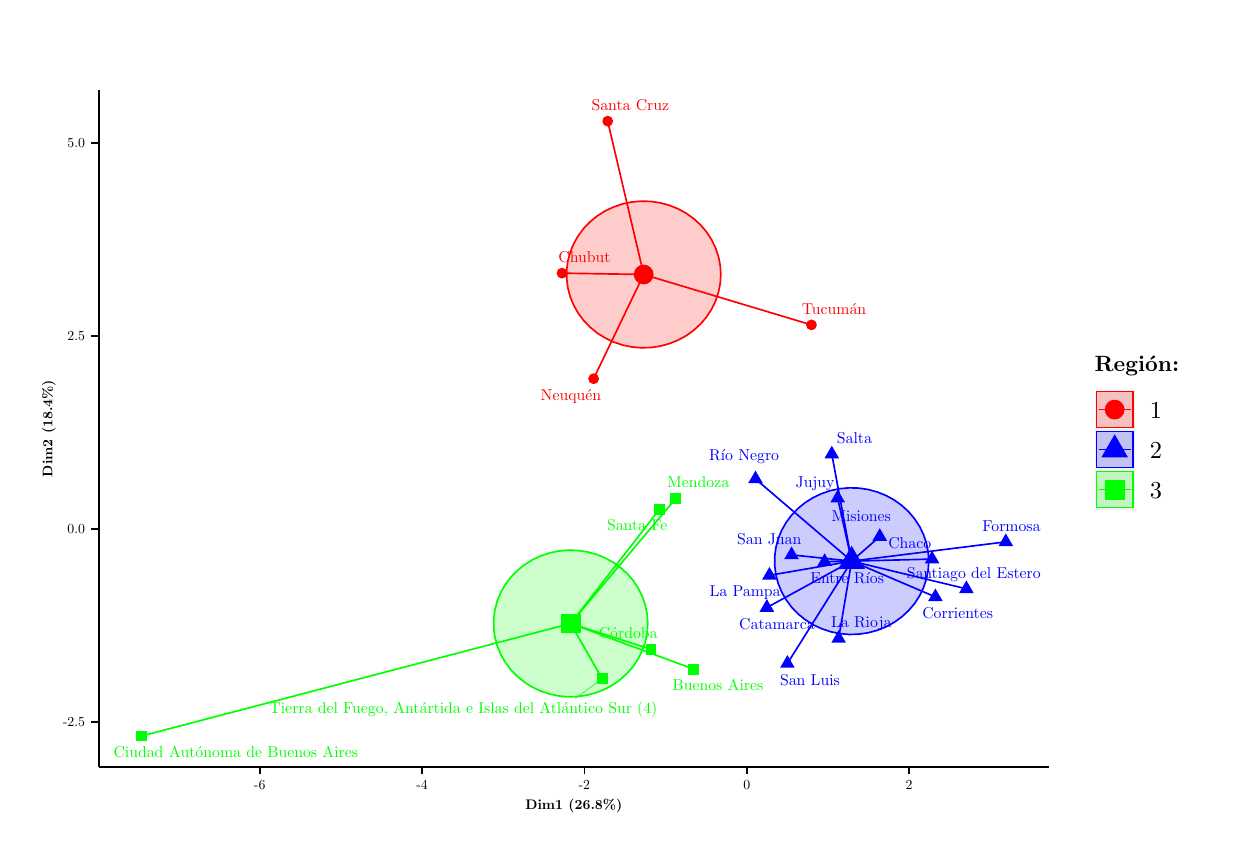
\begin{tikzpicture}[x=1pt,y=1pt]
\definecolor{fillColor}{RGB}{255,255,255}
\path[use as bounding box,fill=fillColor,fill opacity=0.00] (0,0) rectangle (433.62,289.08);
\begin{scope}
\path[clip] (  0.00,  0.00) rectangle (433.62,289.08);
\definecolor{drawColor}{RGB}{255,255,255}
\definecolor{fillColor}{RGB}{255,255,255}

\path[draw=drawColor,line width= 0.6pt,line join=round,line cap=round,fill=fillColor] (  0.00,  0.00) rectangle (433.62,289.08);
\end{scope}
\begin{scope}
\path[clip] ( 25.68, 22.04) rectangle (369.05,266.40);
\definecolor{drawColor}{RGB}{255,255,255}

\path[draw=drawColor,line width= 0.3pt,line join=round] ( 25.68, 73.07) --
	(369.05, 73.07);

\path[draw=drawColor,line width= 0.3pt,line join=round] ( 25.68,142.81) --
	(369.05,142.81);

\path[draw=drawColor,line width= 0.3pt,line join=round] ( 25.68,212.56) --
	(369.05,212.56);

\path[draw=drawColor,line width= 0.3pt,line join=round] ( 54.51, 22.04) --
	( 54.51,266.40);

\path[draw=drawColor,line width= 0.3pt,line join=round] (113.17, 22.04) --
	(113.17,266.40);

\path[draw=drawColor,line width= 0.3pt,line join=round] (171.84, 22.04) --
	(171.84,266.40);

\path[draw=drawColor,line width= 0.3pt,line join=round] (230.50, 22.04) --
	(230.50,266.40);

\path[draw=drawColor,line width= 0.3pt,line join=round] (289.16, 22.04) --
	(289.16,266.40);

\path[draw=drawColor,line width= 0.3pt,line join=round] (347.83, 22.04) --
	(347.83,266.40);

\path[draw=drawColor,line width= 0.6pt,line join=round] ( 25.68, 38.19) --
	(369.05, 38.19);

\path[draw=drawColor,line width= 0.6pt,line join=round] ( 25.68,107.94) --
	(369.05,107.94);

\path[draw=drawColor,line width= 0.6pt,line join=round] ( 25.68,177.69) --
	(369.05,177.69);

\path[draw=drawColor,line width= 0.6pt,line join=round] ( 25.68,247.44) --
	(369.05,247.44);

\path[draw=drawColor,line width= 0.6pt,line join=round] ( 83.84, 22.04) --
	( 83.84,266.40);

\path[draw=drawColor,line width= 0.6pt,line join=round] (142.50, 22.04) --
	(142.50,266.40);

\path[draw=drawColor,line width= 0.6pt,line join=round] (201.17, 22.04) --
	(201.17,266.40);

\path[draw=drawColor,line width= 0.6pt,line join=round] (259.83, 22.04) --
	(259.83,266.40);

\path[draw=drawColor,line width= 0.6pt,line join=round] (318.49, 22.04) --
	(318.49,266.40);
\definecolor{fillColor}{RGB}{0,255,0}

\path[fill=fillColor] ( 39.32, 31.18) --
	( 43.25, 31.18) --
	( 43.25, 35.11) --
	( 39.32, 35.11) --
	cycle;

\path[fill=fillColor] (238.63, 55.34) --
	(242.56, 55.34) --
	(242.56, 59.27) --
	(238.63, 59.27) --
	cycle;
\definecolor{fillColor}{RGB}{0,0,255}

\path[fill=fillColor] (267.10, 82.59) --
	(269.74, 78.01) --
	(264.46, 78.01) --
	cycle;

\path[fill=fillColor] (326.80,100.10) --
	(329.45, 95.52) --
	(324.16, 95.52) --
	cycle;
\definecolor{fillColor}{RGB}{255,0,0}

\path[fill=fillColor] (193.08,200.37) circle (  1.96);
\definecolor{fillColor}{RGB}{0,255,0}

\path[fill=fillColor] (223.28, 62.47) --
	(227.21, 62.47) --
	(227.21, 66.40) --
	(223.28, 66.40) --
	cycle;
\definecolor{fillColor}{RGB}{0,0,255}

\path[fill=fillColor] (328.00, 86.43) --
	(330.65, 81.85) --
	(325.36, 81.85) --
	cycle;

\path[fill=fillColor] (287.99, 99.15) --
	(290.64, 94.58) --
	(285.35, 94.58) --
	cycle;

\path[fill=fillColor] (353.44,106.33) --
	(356.08,101.75) --
	(350.80,101.75) --
	cycle;

\path[fill=fillColor] (292.70,122.14) --
	(295.34,117.56) --
	(290.06,117.56) --
	cycle;

\path[fill=fillColor] (268.04, 94.23) --
	(270.68, 89.65) --
	(265.39, 89.65) --
	cycle;

\path[fill=fillColor] (293.04, 71.40) --
	(295.68, 66.83) --
	(290.40, 66.83) --
	cycle;
\definecolor{fillColor}{RGB}{0,255,0}

\path[fill=fillColor] (232.21,116.98) --
	(236.13,116.98) --
	(236.13,120.91) --
	(232.21,120.91) --
	cycle;
\definecolor{fillColor}{RGB}{0,0,255}

\path[fill=fillColor] (307.90,108.24) --
	(310.54,103.67) --
	(305.26,103.67) --
	cycle;
\definecolor{fillColor}{RGB}{255,0,0}

\path[fill=fillColor] (204.50,162.23) circle (  1.96);
\definecolor{fillColor}{RGB}{0,0,255}

\path[fill=fillColor] (263.00,129.04) --
	(265.64,124.47) --
	(260.35,124.47) --
	cycle;

\path[fill=fillColor] (290.57,138.01) --
	(293.22,133.44) --
	(287.93,133.44) --
	cycle;

\path[fill=fillColor] (276.03,101.62) --
	(278.67, 97.04) --
	(273.38, 97.04) --
	cycle;

\path[fill=fillColor] (274.52, 62.37) --
	(277.16, 57.79) --
	(271.88, 57.79) --
	cycle;
\definecolor{fillColor}{RGB}{255,0,0}

\path[fill=fillColor] (209.59,255.30) circle (  1.96);
\definecolor{fillColor}{RGB}{0,255,0}

\path[fill=fillColor] (226.38,113.13) --
	(230.31,113.13) --
	(230.31,117.05) --
	(226.38,117.05) --
	cycle;
\definecolor{fillColor}{RGB}{0,0,255}

\path[fill=fillColor] (339.20, 89.35) --
	(341.85, 84.77) --
	(336.56, 84.77) --
	cycle;
\definecolor{fillColor}{RGB}{0,255,0}

\path[fill=fillColor] (205.61, 51.82) --
	(209.53, 51.82) --
	(209.53, 55.74) --
	(205.61, 55.74) --
	cycle;
\definecolor{fillColor}{RGB}{255,0,0}

\path[fill=fillColor] (283.22,181.68) circle (  1.96);
\definecolor{drawColor}{RGB}{255,0,0}
\definecolor{fillColor}{RGB}{255,0,0}

\path[draw=drawColor,line width= 0.6pt,line join=round,line cap=round,fill=fillColor,fill opacity=0.20] (250.46,199.89) --
	(250.25,203.15) --
	(249.62,206.36) --
	(248.58,209.47) --
	(247.14,212.43) --
	(245.34,215.21) --
	(243.19,217.75) --
	(240.72,220.02) --
	(237.99,221.99) --
	(235.02,223.62) --
	(231.86,224.89) --
	(228.56,225.78) --
	(225.17,226.29) --
	(221.74,226.39) --
	(218.32,226.08) --
	(214.97,225.39) --
	(211.73,224.30) --
	(208.66,222.85) --
	(205.80,221.04) --
	(203.20,218.92) --
	(200.89,216.51) --
	(198.90,213.85) --
	(197.28,210.97) --
	(196.04,207.93) --
	(195.20,204.76) --
	(194.78,201.53) --
	(194.78,198.26) --
	(195.20,195.02) --
	(196.04,191.86) --
	(197.28,188.82) --
	(198.90,185.94) --
	(200.89,183.28) --
	(203.20,180.87) --
	(205.80,178.74) --
	(208.66,176.94) --
	(211.73,175.49) --
	(214.97,174.40) --
	(218.32,173.70) --
	(221.74,173.40) --
	(225.17,173.50) --
	(228.56,174.00) --
	(231.86,174.90) --
	(235.02,176.17) --
	(237.99,177.80) --
	(240.72,179.77) --
	(243.19,182.04) --
	(245.34,184.58) --
	(247.14,187.36) --
	(248.58,190.32) --
	(249.62,193.43) --
	(250.25,196.64) --
	(250.46,199.89) --
	cycle;
\definecolor{drawColor}{RGB}{0,0,255}
\definecolor{fillColor}{RGB}{0,0,255}

\path[draw=drawColor,line width= 0.6pt,line join=round,line cap=round,fill=fillColor,fill opacity=0.20] (325.60, 96.31) --
	(325.39, 99.56) --
	(324.76,102.77) --
	(323.72,105.88) --
	(322.29,108.84) --
	(320.48,111.62) --
	(318.33,114.16) --
	(315.87,116.43) --
	(313.13,118.40) --
	(310.16,120.03) --
	(307.00,121.30) --
	(303.70,122.20) --
	(300.31,122.70) --
	(296.88,122.80) --
	(293.46,122.50) --
	(290.11,121.80) --
	(286.88,120.71) --
	(283.81,119.26) --
	(280.95,117.46) --
	(278.34,115.33) --
	(276.03,112.92) --
	(274.05,110.26) --
	(272.42,107.38) --
	(271.18,104.34) --
	(270.35,101.18) --
	(269.93, 97.94) --
	(269.93, 94.67) --
	(270.35, 91.44) --
	(271.18, 88.27) --
	(272.42, 85.23) --
	(274.05, 82.35) --
	(276.03, 79.69) --
	(278.34, 77.28) --
	(280.95, 75.16) --
	(283.81, 73.35) --
	(286.88, 71.90) --
	(290.11, 70.81) --
	(293.46, 70.12) --
	(296.88, 69.81) --
	(300.31, 69.92) --
	(303.70, 70.42) --
	(307.00, 71.31) --
	(310.16, 72.58) --
	(313.13, 74.21) --
	(315.87, 76.18) --
	(318.33, 78.45) --
	(320.48, 80.99) --
	(322.29, 83.77) --
	(323.72, 86.73) --
	(324.76, 89.84) --
	(325.39, 93.05) --
	(325.60, 96.31) --
	cycle;
\definecolor{drawColor}{RGB}{0,255,0}
\definecolor{fillColor}{RGB}{0,255,0}

\path[draw=drawColor,line width= 0.6pt,line join=round,line cap=round,fill=fillColor,fill opacity=0.20] (224.07, 73.78) --
	(223.86, 77.04) --
	(223.22, 80.25) --
	(222.18, 83.36) --
	(220.75, 86.32) --
	(218.94, 89.10) --
	(216.79, 91.64) --
	(214.33, 93.91) --
	(211.59, 95.88) --
	(208.62, 97.51) --
	(205.46, 98.78) --
	(202.16, 99.67) --
	(198.77,100.17) --
	(195.34,100.28) --
	(191.93, 99.97) --
	(188.58, 99.28) --
	(185.34, 98.19) --
	(182.27, 96.74) --
	(179.41, 94.93) --
	(176.80, 92.81) --
	(174.49, 90.40) --
	(172.51, 87.74) --
	(170.89, 84.86) --
	(169.65, 81.82) --
	(168.81, 78.65) --
	(168.39, 75.42) --
	(168.39, 72.15) --
	(168.81, 68.91) --
	(169.65, 65.75) --
	(170.89, 62.71) --
	(172.51, 59.83) --
	(174.49, 57.17) --
	(176.80, 54.76) --
	(179.41, 52.63) --
	(182.27, 50.83) --
	(185.34, 49.38) --
	(188.58, 48.29) --
	(191.93, 47.59) --
	(195.34, 47.29) --
	(198.77, 47.39) --
	(202.16, 47.89) --
	(205.46, 48.79) --
	(208.62, 50.06) --
	(211.59, 51.69) --
	(214.33, 53.66) --
	(216.79, 55.93) --
	(218.94, 58.47) --
	(220.75, 61.24) --
	(222.18, 64.21) --
	(223.22, 67.32) --
	(223.86, 70.53) --
	(224.07, 73.78) --
	cycle;
\definecolor{fillColor}{RGB}{255,0,0}

\path[fill=fillColor] (222.60,199.89) circle (  3.57);
\definecolor{fillColor}{RGB}{0,0,255}

\path[fill=fillColor] (297.74,101.86) --
	(302.54, 93.53) --
	(292.93, 93.53) --
	cycle;
\definecolor{fillColor}{RGB}{0,255,0}

\path[fill=fillColor] (192.63, 70.22) --
	(199.77, 70.22) --
	(199.77, 77.35) --
	(192.63, 77.35) --
	cycle;
\definecolor{drawColor}{RGB}{255,0,0}

\path[draw=drawColor,line width= 0.6pt,line join=round] (222.60,199.89) -- (193.08,200.37);

\path[draw=drawColor,line width= 0.6pt,line join=round] (222.60,199.89) -- (204.50,162.23);

\path[draw=drawColor,line width= 0.6pt,line join=round] (222.60,199.89) -- (209.59,255.30);

\path[draw=drawColor,line width= 0.6pt,line join=round] (222.60,199.89) -- (283.22,181.68);
\definecolor{drawColor}{RGB}{0,0,255}

\path[draw=drawColor,line width= 0.6pt,line join=round] (297.74, 96.31) -- (267.10, 79.53);

\path[draw=drawColor,line width= 0.6pt,line join=round] (297.74, 96.31) -- (326.80, 97.05);

\path[draw=drawColor,line width= 0.6pt,line join=round] (297.74, 96.31) -- (328.00, 83.38);

\path[draw=drawColor,line width= 0.6pt,line join=round] (297.74, 96.31) -- (287.99, 96.10);

\path[draw=drawColor,line width= 0.6pt,line join=round] (297.74, 96.31) -- (353.44,103.28);

\path[draw=drawColor,line width= 0.6pt,line join=round] (297.74, 96.31) -- (292.70,119.09);

\path[draw=drawColor,line width= 0.6pt,line join=round] (297.74, 96.31) -- (268.04, 91.18);

\path[draw=drawColor,line width= 0.6pt,line join=round] (297.74, 96.31) -- (293.04, 68.35);

\path[draw=drawColor,line width= 0.6pt,line join=round] (297.74, 96.31) -- (307.90,105.19);

\path[draw=drawColor,line width= 0.6pt,line join=round] (297.74, 96.31) -- (263.00,125.99);

\path[draw=drawColor,line width= 0.6pt,line join=round] (297.74, 96.31) -- (290.57,134.96);

\path[draw=drawColor,line width= 0.6pt,line join=round] (297.74, 96.31) -- (276.03, 98.57);

\path[draw=drawColor,line width= 0.6pt,line join=round] (297.74, 96.31) -- (274.52, 59.32);

\path[draw=drawColor,line width= 0.6pt,line join=round] (297.74, 96.31) -- (339.20, 86.30);
\definecolor{drawColor}{RGB}{0,255,0}

\path[draw=drawColor,line width= 0.6pt,line join=round] (196.20, 73.78) -- ( 41.28, 33.15);

\path[draw=drawColor,line width= 0.6pt,line join=round] (196.20, 73.78) -- (240.60, 57.31);

\path[draw=drawColor,line width= 0.6pt,line join=round] (196.20, 73.78) -- (225.25, 64.44);

\path[draw=drawColor,line width= 0.6pt,line join=round] (196.20, 73.78) -- (234.17,118.94);

\path[draw=drawColor,line width= 0.6pt,line join=round] (196.20, 73.78) -- (228.34,115.09);

\path[draw=drawColor,line width= 0.6pt,line join=round] (196.20, 73.78) -- (207.57, 53.78);

\path[draw=drawColor,line width= 0.2pt,line join=round,line cap=round] (197.76, 46.66) -- (206.77, 53.20);

\node[text=drawColor,anchor=base,inner sep=0pt, outer sep=0pt, scale=  0.57] at ( 75.21, 25.41) {Ciudad Autónoma de Buenos Aires};

\node[text=drawColor,anchor=base,inner sep=0pt, outer sep=0pt, scale=  0.57] at (249.45, 49.50) {Buenos Aires};
\definecolor{drawColor}{RGB}{0,0,255}

\node[text=drawColor,anchor=base,inner sep=0pt, outer sep=0pt, scale=  0.57] at (270.75, 71.71) {Catamarca};

\node[text=drawColor,anchor=base,inner sep=0pt, outer sep=0pt, scale=  0.57] at (318.76,100.80) {Chaco};
\definecolor{drawColor}{RGB}{255,0,0}

\node[text=drawColor,anchor=base,inner sep=0pt, outer sep=0pt, scale=  0.57] at (201.19,204.21) {Chubut};
\definecolor{drawColor}{RGB}{0,255,0}

\node[text=drawColor,anchor=base,inner sep=0pt, outer sep=0pt, scale=  0.57] at (217.01, 68.29) {Córdoba};
\definecolor{drawColor}{RGB}{0,0,255}

\node[text=drawColor,anchor=base,inner sep=0pt, outer sep=0pt, scale=  0.57] at (336.06, 75.64) {Corrientes};

\node[text=drawColor,anchor=base,inner sep=0pt, outer sep=0pt, scale=  0.57] at (296.12, 88.38) {Entre Ríos};

\node[text=drawColor,anchor=base,inner sep=0pt, outer sep=0pt, scale=  0.57] at (355.50,107.09) {Formosa};

\node[text=drawColor,anchor=base,inner sep=0pt, outer sep=0pt, scale=  0.57] at (284.53,122.97) {Jujuy};

\node[text=drawColor,anchor=base,inner sep=0pt, outer sep=0pt, scale=  0.57] at (259.23, 83.42) {La Pampa};

\node[text=drawColor,anchor=base,inner sep=0pt, outer sep=0pt, scale=  0.57] at (301.23, 72.19) {La Rioja};
\definecolor{drawColor}{RGB}{0,255,0}

\node[text=drawColor,anchor=base,inner sep=0pt, outer sep=0pt, scale=  0.57] at (242.33,122.78) {Mendoza};
\definecolor{drawColor}{RGB}{0,0,255}

\node[text=drawColor,anchor=base,inner sep=0pt, outer sep=0pt, scale=  0.57] at (301.21,110.80) {Misiones};
\definecolor{drawColor}{RGB}{255,0,0}

\node[text=drawColor,anchor=base,inner sep=0pt, outer sep=0pt, scale=  0.57] at (196.30,154.45) {Neuquén};
\definecolor{drawColor}{RGB}{0,0,255}

\node[text=drawColor,anchor=base,inner sep=0pt, outer sep=0pt, scale=  0.57] at (258.89,132.83) {Río Negro};

\node[text=drawColor,anchor=base,inner sep=0pt, outer sep=0pt, scale=  0.57] at (298.77,138.88) {Salta};

\node[text=drawColor,anchor=base,inner sep=0pt, outer sep=0pt, scale=  0.57] at (267.96,102.39) {San Juan};

\node[text=drawColor,anchor=base,inner sep=0pt, outer sep=0pt, scale=  0.57] at (282.70, 51.52) {San Luis};
\definecolor{drawColor}{RGB}{255,0,0}

\node[text=drawColor,anchor=base,inner sep=0pt, outer sep=0pt, scale=  0.57] at (217.77,259.19) {Santa Cruz};
\definecolor{drawColor}{RGB}{0,255,0}

\node[text=drawColor,anchor=base,inner sep=0pt, outer sep=0pt, scale=  0.57] at (220.26,107.35) {Santa Fe};
\definecolor{drawColor}{RGB}{0,0,255}

\node[text=drawColor,anchor=base,inner sep=0pt, outer sep=0pt, scale=  0.57] at (341.87, 90.14) {Santiago del Estero};
\definecolor{drawColor}{RGB}{0,255,0}

\node[text=drawColor,anchor=base,inner sep=0pt, outer sep=0pt, scale=  0.57] at (157.46, 41.24) {Tierra del Fuego, Antártida e Islas del Atlántico Sur (4)};
\definecolor{drawColor}{RGB}{255,0,0}

\node[text=drawColor,anchor=base,inner sep=0pt, outer sep=0pt, scale=  0.57] at (291.38,185.56) {Tucumán};
\end{scope}
\begin{scope}
\path[clip] (  0.00,  0.00) rectangle (433.62,289.08);
\definecolor{drawColor}{RGB}{0,0,0}

\path[draw=drawColor,line width= 0.6pt,line join=round] ( 25.68, 22.04) --
	( 25.68,266.40);
\end{scope}
\begin{scope}
\path[clip] (  0.00,  0.00) rectangle (433.62,289.08);
\definecolor{drawColor}{RGB}{0,0,0}

\node[text=drawColor,anchor=base east,inner sep=0pt, outer sep=0pt, scale=  0.50] at ( 20.73, 36.47) {-2.5};

\node[text=drawColor,anchor=base east,inner sep=0pt, outer sep=0pt, scale=  0.50] at ( 20.73,106.22) {0.0};

\node[text=drawColor,anchor=base east,inner sep=0pt, outer sep=0pt, scale=  0.50] at ( 20.73,175.97) {2.5};

\node[text=drawColor,anchor=base east,inner sep=0pt, outer sep=0pt, scale=  0.50] at ( 20.73,245.71) {5.0};
\end{scope}
\begin{scope}
\path[clip] (  0.00,  0.00) rectangle (433.62,289.08);
\definecolor{drawColor}{RGB}{0,0,0}

\path[draw=drawColor,line width= 0.6pt,line join=round] ( 22.93, 38.19) --
	( 25.68, 38.19);

\path[draw=drawColor,line width= 0.6pt,line join=round] ( 22.93,107.94) --
	( 25.68,107.94);

\path[draw=drawColor,line width= 0.6pt,line join=round] ( 22.93,177.69) --
	( 25.68,177.69);

\path[draw=drawColor,line width= 0.6pt,line join=round] ( 22.93,247.44) --
	( 25.68,247.44);
\end{scope}
\begin{scope}
\path[clip] (  0.00,  0.00) rectangle (433.62,289.08);
\definecolor{drawColor}{RGB}{0,0,0}

\path[draw=drawColor,line width= 0.6pt,line join=round] ( 25.68, 22.04) --
	(369.05, 22.04);
\end{scope}
\begin{scope}
\path[clip] (  0.00,  0.00) rectangle (433.62,289.08);
\definecolor{drawColor}{RGB}{0,0,0}

\path[draw=drawColor,line width= 0.6pt,line join=round] ( 83.84, 19.29) --
	( 83.84, 22.04);

\path[draw=drawColor,line width= 0.6pt,line join=round] (142.50, 19.29) --
	(142.50, 22.04);

\path[draw=drawColor,line width= 0.6pt,line join=round] (201.17, 19.29) --
	(201.17, 22.04);

\path[draw=drawColor,line width= 0.6pt,line join=round] (259.83, 19.29) --
	(259.83, 22.04);

\path[draw=drawColor,line width= 0.6pt,line join=round] (318.49, 19.29) --
	(318.49, 22.04);
\end{scope}
\begin{scope}
\path[clip] (  0.00,  0.00) rectangle (433.62,289.08);
\definecolor{drawColor}{RGB}{0,0,0}

\node[text=drawColor,anchor=base,inner sep=0pt, outer sep=0pt, scale=  0.50] at ( 83.84, 13.64) {-6};

\node[text=drawColor,anchor=base,inner sep=0pt, outer sep=0pt, scale=  0.50] at (142.50, 13.64) {-4};

\node[text=drawColor,anchor=base,inner sep=0pt, outer sep=0pt, scale=  0.50] at (201.17, 13.64) {-2};

\node[text=drawColor,anchor=base,inner sep=0pt, outer sep=0pt, scale=  0.50] at (259.83, 13.64) {0};

\node[text=drawColor,anchor=base,inner sep=0pt, outer sep=0pt, scale=  0.50] at (318.49, 13.64) {2};
\end{scope}
\begin{scope}
\path[clip] (  0.00,  0.00) rectangle (433.62,289.08);
\definecolor{drawColor}{RGB}{0,0,0}

\node[text=drawColor,anchor=base,inner sep=0pt, outer sep=0pt, scale=  0.50] at (197.36,  6.47) {\bfseries Dim1 (26.8{\%})};
\end{scope}
\begin{scope}
\path[clip] (  0.00,  0.00) rectangle (433.62,289.08);
\definecolor{drawColor}{RGB}{0,0,0}

\node[text=drawColor,rotate= 90.00,anchor=base,inner sep=0pt, outer sep=0pt, scale=  0.50] at (  8.95,144.22) {\bfseries Dim2 (18.4{\%})};
\end{scope}
\begin{scope}
\path[clip] (  0.00,  0.00) rectangle (433.62,289.08);
\definecolor{fillColor}{RGB}{255,255,255}

\path[fill=fillColor] (380.05,109.43) rectangle (428.12,179.02);
\end{scope}
\begin{scope}
\path[clip] (  0.00,  0.00) rectangle (433.62,289.08);
\definecolor{drawColor}{RGB}{0,0,0}

\node[text=drawColor,anchor=base west,inner sep=0pt, outer sep=0pt, scale=  0.8] at (385.55,164.86) {\bfseries Región:};
\end{scope}
\begin{scope}
\path[clip] (  0.00,  0.00) rectangle (433.62,289.08);
\definecolor{fillColor}{gray}{0.95}

\path[fill=fillColor] (385.55,143.83) rectangle (400.00,158.29);
\end{scope}
\begin{scope}
\path[clip] (  0.00,  0.00) rectangle (433.62,289.08);
\definecolor{fillColor}{RGB}{255,0,0}

\path[fill=fillColor] (392.78,151.06) circle (  1.96);
\end{scope}
\begin{scope}
\path[clip] (  0.00,  0.00) rectangle (433.62,289.08);
\definecolor{drawColor}{RGB}{255,0,0}
\definecolor{fillColor}{RGB}{255,0,0}

\path[draw=drawColor,line width= 0.6pt,line cap=rect,fill=fillColor,fill opacity=0.20] (386.26,144.54) rectangle (399.29,157.58);
\end{scope}
\begin{scope}
\path[clip] (  0.00,  0.00) rectangle (433.62,289.08);
\definecolor{fillColor}{RGB}{255,0,0}

\path[fill=fillColor] (392.78,151.06) circle (  3.57);
\end{scope}
\begin{scope}
\path[clip] (  0.00,  0.00) rectangle (433.62,289.08);
\definecolor{drawColor}{RGB}{255,0,0}

\path[draw=drawColor,line width= 0.6pt,line join=round] (386.99,151.06) -- (398.56,151.06);
\end{scope}
\begin{scope}
\path[clip] (  0.00,  0.00) rectangle (433.62,289.08);
\definecolor{drawColor}{RGB}{255,0,0}

\node[text=drawColor,anchor=base,inner sep=0pt, outer sep=0pt, scale=  0.57] at (392.78,149.10) {a};
\end{scope}
\begin{scope}
\path[clip] (  0.00,  0.00) rectangle (433.62,289.08);
\definecolor{fillColor}{gray}{0.95}

\path[fill=fillColor] (385.55,129.38) rectangle (400.00,143.83);
\end{scope}
\begin{scope}
\path[clip] (  0.00,  0.00) rectangle (433.62,289.08);
\definecolor{fillColor}{RGB}{0,0,255}

\path[fill=fillColor] (392.78,139.66) --
	(395.42,135.08) --
	(390.13,135.08) --
	cycle;
\end{scope}
\begin{scope}
\path[clip] (  0.00,  0.00) rectangle (433.62,289.08);
\definecolor{drawColor}{RGB}{0,0,255}
\definecolor{fillColor}{RGB}{0,0,255}

\path[draw=drawColor,line width= 0.6pt,line cap=rect,fill=fillColor,fill opacity=0.20] (386.26,130.09) rectangle (399.29,143.12);
\end{scope}
\begin{scope}
\path[clip] (  0.00,  0.00) rectangle (433.62,289.08);
\definecolor{fillColor}{RGB}{0,0,255}

\path[fill=fillColor] (392.78,142.16) --
	(397.58,133.83) --
	(387.97,133.83) --
	cycle;
\end{scope}
\begin{scope}
\path[clip] (  0.00,  0.00) rectangle (433.62,289.08);
\definecolor{drawColor}{RGB}{0,0,255}

\path[draw=drawColor,line width= 0.6pt,line join=round] (386.99,136.61) -- (398.56,136.61);
\end{scope}
\begin{scope}
\path[clip] (  0.00,  0.00) rectangle (433.62,289.08);
\definecolor{drawColor}{RGB}{0,0,255}

\node[text=drawColor,anchor=base,inner sep=0pt, outer sep=0pt, scale=  0.57] at (392.78,134.65) {a};
\end{scope}
\begin{scope}
\path[clip] (  0.00,  0.00) rectangle (433.62,289.08);
\definecolor{fillColor}{gray}{0.95}

\path[fill=fillColor] (385.55,114.93) rectangle (400.00,129.38);
\end{scope}
\begin{scope}
\path[clip] (  0.00,  0.00) rectangle (433.62,289.08);
\definecolor{fillColor}{RGB}{0,255,0}

\path[fill=fillColor] (390.81,120.19) --
	(394.74,120.19) --
	(394.74,124.11) --
	(390.81,124.11) --
	cycle;
\end{scope}
\begin{scope}
\path[clip] (  0.00,  0.00) rectangle (433.62,289.08);
\definecolor{drawColor}{RGB}{0,255,0}
\definecolor{fillColor}{RGB}{0,255,0}

\path[draw=drawColor,line width= 0.6pt,line cap=rect,fill=fillColor,fill opacity=0.20] (386.26,115.64) rectangle (399.29,128.67);
\end{scope}
\begin{scope}
\path[clip] (  0.00,  0.00) rectangle (433.62,289.08);
\definecolor{fillColor}{RGB}{0,255,0}

\path[fill=fillColor] (389.21,118.58) --
	(396.34,118.58) --
	(396.34,125.72) --
	(389.21,125.72) --
	cycle;
\end{scope}
\begin{scope}
\path[clip] (  0.00,  0.00) rectangle (433.62,289.08);
\definecolor{drawColor}{RGB}{0,255,0}

\path[draw=drawColor,line width= 0.6pt,line join=round] (386.99,122.15) -- (398.56,122.15);
\end{scope}
\begin{scope}
\path[clip] (  0.00,  0.00) rectangle (433.62,289.08);
\definecolor{drawColor}{RGB}{0,255,0}

\node[text=drawColor,anchor=base,inner sep=0pt, outer sep=0pt, scale=  0.57] at (392.78,120.19) {a};
\end{scope}
\begin{scope}
\path[clip] (  0.00,  0.00) rectangle (433.62,289.08);
\definecolor{drawColor}{RGB}{0,0,0}

\node[text=drawColor,anchor=base west,inner sep=0pt, outer sep=0pt, scale=  0.88] at (405.50,148.03) {1};
\end{scope}
\begin{scope}
\path[clip] (  0.00,  0.00) rectangle (433.62,289.08);
\definecolor{drawColor}{RGB}{0,0,0}

\node[text=drawColor,anchor=base west,inner sep=0pt, outer sep=0pt, scale=  0.88] at (405.50,133.58) {2};
\end{scope}
\begin{scope}
\path[clip] (  0.00,  0.00) rectangle (433.62,289.08);
\definecolor{drawColor}{RGB}{0,0,0}

\node[text=drawColor,anchor=base west,inner sep=0pt, outer sep=0pt, scale=  0.88] at (405.50,119.12) {3};
\end{scope}
\end{tikzpicture}
